\documentclass[12pt]{unlsilabsop}

\title{Master SOP}
\date{June 27, 2014}
\author{Frank Meier Aeschbacher}
\approved{Frank Meier Aeschbacher}
\sopid{000}
\sopversion{v0}
\sopabstract{This master document describes the operations at UNL for manufacturing and testing modules within the \emph{CMS Pixel Phase-I} upgrade project. It describes responsibilities, local organization and the documentation structure.}
\begin{document}

\maketitle

\section{Scope}
The high energy physics group at University of Nebraska-Lincoln hosts one of the two US manufacturing sites for sensor modules to be used in the upgraded CMS forward pixel detector. 

\section{Purpose}
This document and the herein listed subdocuments describe the procedures in place to manufacture modules to high standards and principles to assure their quality.

\section{Definitions}
The definitions defined here apply to all subdocuments as well.
\begin{description}
    \item[BBM] \emph{Bare bump-bonded module.} Consists of a silicon sensor and 16 ROC, attached through bump bonding.
    \item[HDI] \emph{High-Density Interconnect}. Flexible circuit board providing connection from the ROC to the data acquisition systems. Contains a TBM
    \item[ROC] \emph{Read Out Chip.} Chips attached to the sensors using bump bonding. Every pixel of the sensor is attached to an individual amplifier/comparator circuit on the ROC, which orchestrates the readout of signals for all pixels covered by one ROC.
    \item[TBM] \emph{Token Bit Manager.} Chip to control the readout of ROC in a module and providing interfaces to the outer world. Normally part of an HDI.
\end{description}

\section{Responsibilities}

\section{Document hierarchy}
The documents are organised in a hierarchical way, as outlined by Fig.~\ref{fig:SOPhierarchy}.
\begin{figure}[h]
    \begin{center}
        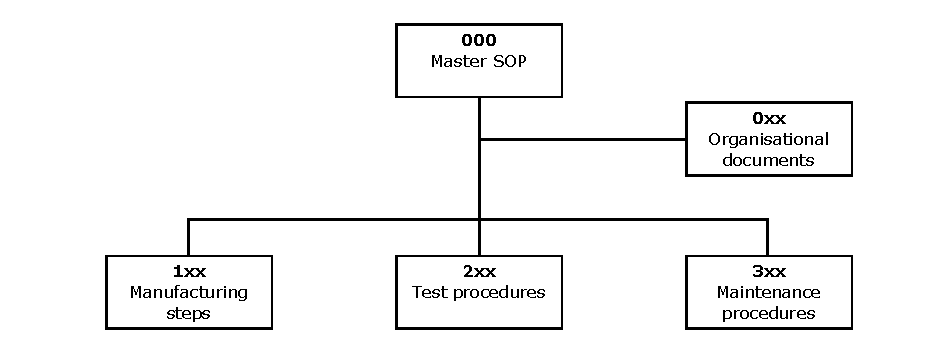
\includegraphics[width=16cm]{img/SOPhierarchy.pdf}
        \caption{Hierachy of SOP documents. The thre-digt number identifies documents and the first digit assigns it to a class.}
        \label{fig:SOPhierarchy}
    \end{center}
\end{figure}
Documents are identified by a 3-digit number. The top-level document has the number 000. All the other documents carry numbers different from this. The first digit identifies the group the document belongs to, see figure.

\subsection{Versioning of documents}
Any SOP document carries a revision number, consisting of the letter `v' followed by a number. `v0' identifies a draft document. Any document `v1' and above is effective as of the date printed.

\subsection{List of documents}
Table \ref{tbl:SOPlist} shows the planned documents. They do not need to be in place before this document becomes v1. A list of all current documents is to be maintained and made accessible to all people involved.

\begin{table*}[hH]
\begin{center}
\caption{List of SOP documents}
\label{tbl:SOPlist}

\bigskip

{\footnotesize
\begin{tabular}{lp{7cm}p{6cm}}
\toprule
No. & Title & Comment \\
\midrule
000 & Master SOP & This document \\
\midrule
001 & Production cycle and quality control & General process description \\
002 & General documentation procedures & \\
003 & Training & \\
004 & Access control & \\
005 & Backup and recovery & \\
006 & Protective measures & Personal protection, clean room rules, environmental protection \\
\midrule
101 & Deliveries of HDI & \\
102 & Deliveries of BBM & \\
103 & Glueing of HDI to BBM & \\
104 & Wirebonding of modules & \\
105 & Encapsulation of wirebonds & \\
106 & Final inspection and shipping of modules & \\
107 & Reworking of modules & \\
\midrule
201 & Visual inspection of HDI & \\
202 & Visual inspection of BBM & \\
203 & IV test of BBM & \\
204 & Electrical acceptance test of HDI & \\
205 & Visual inspection of final module & \\
206 & Electrical acceptance test of final module & \\
207 & Pull testing of wirebonds & \\
208 & Electrical acceptance test of BBM & \\
\midrule
301 & Cleanroom & \\
302 & Gantry & Covers glueing and encapsulation \\
303 & Wirebonder and pull tester & \\
304 & Probe station & \\
305 & Vacuum supply & \\
306 & Dry air supply & \\
307 & Cold box & \\
\bottomrule
\end{tabular}
}
\end{center}
\end{table*}


\section{Production life-cycle and critical control points}

\section{Documentation of workflow, test results and maintenance operations}

\section{Training}

\end{document}

